\chapter{Modellierungen und Ergebnisse}
\label{ch:ergebnisse}

Die Modellierungen und Ergebnisse dieser Arbeit stützen sich auf die vorgestellten theoretischen Inhalte und werden in den folgenden Abschnitten dargelegt.
Im ersten Teil werden die in Kapitel \ref{ch:isolatormodelle} behandelten Modelle auf ein mikroskopisches, zweidimensionales, quadratisches Festkörpersystem, bestehend aus vier Gitterplätzen, angewandt.
Da jeder Gitterplatz zwei direkte Nachbarn besitzt, kann das Festkörpersystem für ortsunabhängige Betrachtungen auch als eindimensionale Kette mit periodischen Randbedingungen interpretiert werden.
Im zweiten Teil dieses Kapitels wird der in Kapitel \ref{ch:ife} vorgestellte IFE in einem Mott-Hubbard-Isolator untersucht.

Die Darstellung von Vielteilchenzuständen in erster Quantisierung aus Gleichung \eqref{eqn:vtdarstellung1quant} wird im Folgenden mit
\begin{align}
  \ket{\Psi} = \ket{k_1,...,k_{N_e}}
  \label{eqn:vtdarstellung1quantkurz}
\end{align}
abgekürzt. Bei allen Summierungen über Gitterplätze sind periodische Randbedingungen vorausgesetzt.
Numerische Diagonalisierungen von Matrizen werden mit der Funktion \textit{eig} von \textit{GNU Octave} durchgeführt.
Zum Lösen von Differentialgleichungen werden die Integrationsverfahren Runge-Kutta-5 und Runge-Kutta-8 der Funktion \textit{complex\_ode} von \textit{scipy.integrate} verwendet.
Die Werte der verwendeten Naturkonstanten $\symup{e}, \hbar, c$ und $\epsilon_0$ werden dem Lehrbuch \cite{kittel} entnommen.

\section{Analyse eines Festkörpersystems im Tight-Binding-Modell}
\label{sec:untersuchungtb}

In diesem Abschnitt wird die Dynamik eines Festkörpersystems, bestehend aus vier Niveaus, die jeweils einen Gitterplatz repräsentieren, und einem bzw. zwei Elektronen (im Folgenden abgekürzt mit 4N1E bzw. 4N2E),
im Tight-Binding-Modell analysiert. Das 4N1E-System ist in Abbildung \ref{fig:vierniveausystem} mit beispielhafter Besetzung skizziert.
\begin{figure}
  \centering
  \includegraphics[height = 3.2cm]{Graphiken/vier_niveau_system.pdf}
  \caption{Skizze des 4N1E-Systems mit beispielhafter Besetzung $\ket{3}$. Die waagerechten Striche stellen die Niveaus dar, die eingekreisten Zahlen die Nummer des Gitterplatzes, der rot gefärbte Kreis das Elektron
  und die Pfeile die möglichen Sprünge des Elektrons aus der dargestellten Besetzung in Abhängigkeit von $J$.}
  \label{fig:vierniveausystem}
\end{figure}
Das eine Elektron kann in Abhängigkeit von der Tight-Binding-Stärke $J$ waagerecht oder senkrecht zwischen den Gitterplätzen springen.
Der Hilbertraum des 4N1E-Systems setzt sich aus vier Basis-Zuständen, bei denen sich das Elektron jeweils auf einem der vier Gitterplätze befindet, zusammen und ist daher vierdimensional.
Um die Dynamik zu analysieren werden zuerst die Basis-Zustände aufgestellt, daraus die vierdimensionale Hamilton-Matrix bestimmt und mit Hilfe dieser die Schrödingergleichung \eqref{eqn:schroedingergleichung} gelöst.

Zur Darstellung der Basis-Zustände wird die Konvention
\begin{align}
  \ket{i} = \ket{f_i(x)}
  \label{eqn:4N1Ezustandsvorschrift}
\end{align}
verwendet. Dabei gibt die Funktion $f_i(x)$ die Nummer des Gitterplatzes an, auf dem sich das Elektron $x$ befindet.
Der Hamiltonoperator des Systems ist in Gleichung \eqref{eqn:hamiltontb} in zweiter Quantisierung angegeben.
In Tabelle \ref{tab:4N1Ezust} sind die Basis-Zustände und in Gleichung \eqref{eqn:4N1Ehamiltonmatrix} die Matrixdarstellung des Hamiltonoperators $H$, die sich aus Gleichung \eqref{eqn:matrixelemente} ergibt, dargestellt.
Damit wird die stationäre Schrödingergleichung \eqref{eqn:statschroedinger} aufgestellt und durch Diagonalisieren der Hamilton-Matrix analytisch gelöst.
Die berechneten Energie-Eigenwerte $E_q/J$ und die Koeffizienten $\alpha_{i,q}$ der generierten Eigenzustände $\Psi_q$ sind in Tabelle \ref{tab:4N1Eeig} aufgelistet.
Die Eigenzustände ergeben sich aus der Linearkombination
\begin{align}
  \Psi_q = \sum_i \alpha_{i,q} \ket{i}.
  \label{eqn:linkomb}
\end{align}
Da das Betragsquadrat der Koeffizienten $\alpha_{i,q}$ jeweils der Besetzungswahrscheinlichkeit $P_i \in [0,1]$ für den i-ten Basis-Zustand des Systems im Eigenzustand $\Psi_q$ entspricht,
ist an die Linearkombination \eqref{eqn:linkomb} die Normierungsbedingung
\begin{align}
  \sum_i \lvert \alpha_{i,q} \rvert^2 = 1.
  \label{eqn:tbnb}
\end{align}
geknüpft.
\begin{table}[h]
  \centering
  \caption{Analytisch berechnete Eigenwerte $E_q/J$ und zugehörige Koeffizienten $\alpha_{i,q}/0.5$ der Eigenzustände $\Psi_q$ des 4N1E-Systems.}
  \begin{tabular}{S[table-format=1.0] S[table-format=2.0] S[table-format=1.0] S[table-format=1.0] S[table-format=1.0] S[table-format=2.0]}
    \toprule
    {$q$} & {$E_q/J$} & {$\alpha_{1,q}/0.5$} & {$\alpha_{2,q}/0.5$} & {$\alpha_{3,q}/0.5$} & {$\alpha_{4,q}/0.5$}\\
    \midrule
    0 & -2 & 1          & 1          & 1                  & 1                  \\
    1 & 0  & $\sqrt{2}$ & 0          & \text{$-\sqrt{2}$} & 0                  \\
    2 & 0  & 0          & $\sqrt{2}$ & 0                  & \text{$-\sqrt{2}$} \\
    3 & 2  & 1          & -1         & 1                  & -1                 \\
    \bottomrule
  \end{tabular}
  \label{tab:4N1Eeig}
\end{table}
Die Erwartung ist dadurch bestätigt, dass die Eigenenergien $E_q$ in der für das Tight-Binding-Modell vorausgesagten Bandbreite $W = 4J$ der Dispersionsrelation \eqref{eqn:dispersion} liegen.

%Die einzige Quantenzahl, in denen sich die Basis-Zustände des 4N1E-Systems unterscheiden, ist die Nummer $i$ des Gitterplatzes, an welchem das Elektron positioniert ist.
%Da alle Gitterplätze jeweils zwei direkte Nachbarn besitzen, die sich bis auf die Nummer $i$ nicht unterscheiden,
%ist die Besetzungswahrscheinlichkeit des Elektrons in den Eigenzuständen, die sich aus nicht-entarteten Eigen-Energien ergeben, gleichmäßig auf alle vier Basis-Zustände bzw. Niveaus aufgeteilt.
%Aus der Normierungsbedingung \eqref{eqn:tnbn} folgt daher für diese Eigenzustände des Systems
%\begin{align}
%  P_{i,k} = \lvert \alpha_{i,k} \rvert^2 = 0.25.
%  \label{eqn:BesetzungRot}
%\end{align}
%Das ist für die berechneten Eigenzustände $v_0$ und $v_3$ der Fall. Für die Eigenzustände zu entarteten Energie-Eigenwerten, hier $v_1$ und $v_2$ zur Energie $E_1 = E_2 = 0$, können mehrere verschiedene
%Basen gewählt werden, sodass Gleichung \eqref{eqn:BesetzungRot} nicht zwangsläufig gilt. Der physikalische Grund dafür ist, dass das Elektron bei hinreichender Energie einen Zustand,
%der sich aus einer Linearkombination der beiden Eigenzustände $v_1$ und $v_2$ ergibt, besetzt.

Um den Einfluss der Pauli-Wechselwirkung zu untersuchen, werden im nächsten Schritt die Eigenenergien eines 4N2E-Systems bestimmt.
In diesem System sind die waagerechten und senkrechten Sprünge der Elektronen zwichen den Gitterplätzen durch das Pauliprinzip eingeschränkt,
da die Doppelbesetzung eines Niveaus verhindert wird. Für das 4N2E-System ergeben sich insgesamt
\begin{align*}
  \binom{d_{\text{1e}}}{N_e} = \binom42 = 6
\end{align*}
verschiedene Basis-Zustände, wobei $d_\text{1e}$ die Hilbertraum-Dimension des 4N1E-Systems und $N_e$ die Anzahl an Elektronen ist.
Die Eigenenergien setzen sich jeweils additiv aus zwei, aufgrund des Pauliprinzips unterschiedlichen, Eigenenergien des 4N1E-Systems zusammen.
In Tabelle \ref{tab:4N2Eeigenwerte} sind die addierten Eigenenergien für das 4N2E-System aufgelistet. Auch diese liegen in der in Abschnitt \ref{sec:hubbardmodell}
vorrausgesagten Bandbreite $W = 4J$.

\begin{table}[h]
  \centering
  \caption{Additiv aus den Eigenenergien $E_q$ des 4N1E-Systems in Tabelle \ref{tab:4N1Eeig} berechnete Eigenenergien des 4N2E-Systems in Einheiten von $J$.}
  \begin{tabular}{S[table-format=2.0] S[table-format=2.0] S[table-format=1.0] S[table-format=1.0] S[table-format=1.0] S[table-format=1.0]}
    \toprule
    {$E_0/J$} & {$E_1/J$} & {$E_2/J$} & {$E_3/J$} & {$E_4/J$} & {$E_5/J$}\\
    \midrule
    -2 & -2 & 0 & 0 & 2 & 2 \\
    \bottomrule
  \end{tabular}
  \label{tab:4N2Eeigenwerte}
\end{table}

Auf Grundlage der vorgestellten Vierniveausysteme wird im Folgenden ein Mott-Hubbard-Isolator modelliert, indem die atomaren Niveaus des
beschriebenen Gittersystems jeweils in ein Spin-Up- und ein Spin-Down-Niveau aufgespalten werden.

\section{Untersuchung eines Mott-Hubbard-Isolators}
\label{sec:untersuchunghubb}

In diesem Abschnitt wird die Dynamik eines Mott-Isolators, bestehend aus vier Gitterplätzen und acht Niveaus, im Hubbard-Modell untersucht.
Jeder Gitterplatz besitzt zwei Niveaus, die sich jeweils in der Spinausrichtung $\sigma$ unterscheiden.
Auf jeweils vier Niveaus mit äquvalenter Spinausrichtung sind zwei Elektronen verteilt, sodass das System (im Folgenden mit 8N4E abgekürzt) insgesamt halbgefüllt ist.
In Abbildung \ref{fig:hubbsystem} ist eine Skizze des Systems mit beispielhafter Elektronenbesetzung abgebildet.
Die Elektronen können unter Beachtung des Pauliprinzips waagerecht oder senkrecht zwischen den Gitterplätzen auf dem jeweiligen Spin-Niveau springen.
Das 8N4E-System besteht effektiv aus zwei gekoppelten 4N2E-Systemen mit unterschiedlicher Spinausrichtung und
beinhaltet daher $6 \cdot 6=36$ Basis-Zustände bzw. umfasst einen 36D-Hilbertraum.
Mit Hilfe der Kurzschreibweise der Vielteilchenzustände \eqref{eqn:vtdarstellung1quantkurz} werden die Basis-Zustände des Systems in erster Quantisierung in dem Schema
\begin{align}
  \ket{i} = \ket{f_i(\uparrow_1),f_i(\uparrow_2); f_i(\downarrow_1),f_i(\downarrow_2)}
  \label{eqn:8N4Ezustandsvorschrift}
\end{align}
dargestellt. Dabei ist $f_i(x_\alpha)$ eine Funktion, welche den Ort des Elektrons $x_\alpha$ im i-ten Basis-Zustand des Systems angibt.
In der Bezeichnung des Elektrons $x_\alpha$ stellt $x$ die Spinausrichtung und der Index $\alpha$ die Nummer des Elektrons dar, wobei die Elektronen eines Spinniveaus gegen den Uhrzeigersinn und beginnend beim Gitterplatz $1$ durchnummeriert werden.
Diese Konvention führt automatisch dazu, dass der zweite Eintrag einer Spinausrichtung in der Darstellung der Zustände \eqref{eqn:8N4Ezustandsvorschrift} größer als der erste ist.

\begin{figure}
  \centering
  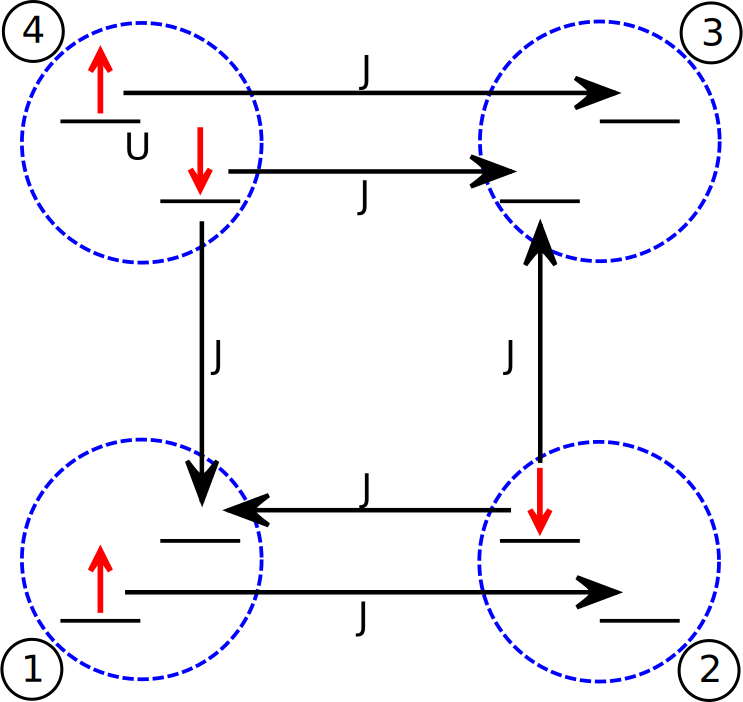
\includegraphics[height = 5.8cm]{Graphiken/hubbard_system.pdf}
  \caption{Skizze des 8N4E-Systems zur Modellierung eines Mott-Hubbard-Isolators. Die blau gestrichelten Kreise umfassen jeweils einen Gitterplatz mit zwei Niveaus
  für die jeweilige Spinausrichtung. Die roten Pfeile stellen die Elektronen inklusive ihre Spinausrichtung dar. Die Elektronen können aus der dargestellten Besetzung $\ket{1,4;2,4}$
  jeweils abhängig von $U$ und $J$ in Pfeilrichtung springen.}
  \label{fig:hubbsystem}
\end{figure}

Die Darstellungen der $36$ Basis-Zustände mit der Vorschrift \eqref{eqn:8N4Ezustandsvorschrift} sind in Tabelle \ref{tab:8N4Ehubbzust} aufgelistet.
Der Hamiltonoperator des 8N4E-Systems ist in Gleichung \eqref{eqn:hamiltonhubb} angegeben.
Um die stationäre Schrödingergleichung für das System zu lösen, wird die $36 \times 36$ - Matrix des Hamiltonoperators analog zu Abschnitt \ref{sec:untersuchungtb} aufgestellt.
Dabei bestimmt die Tight-Binding-Stärke $J$ die Nichtdiagonalelemente und der Hubbard-Parameter $U$ die Diagonalelemente der Matrix.
Diese ist in Gleichung \eqref{eqn:8N4Ehubbmatrix} angegeben.
Die vier niedrigsten Eigenenergiewerte des 8N4E-Systems sind in Tabelle \ref{tab:eigenwerte} in Einheiten von $J$ für diverse $U/J$ aufsteigend aufgelistet und in Abbildung \ref{fig:eplot} gegen $U/J$ graphisch aufgetragen.
Im Grenzfall für den Hubbard-Parameter $U/J = 0$ verschwindet die Coulomb-Wechselwirkung der Elektronen untereinander, sodass sich die 36 Eigenenergien des 8N4E-Systems additiv aus den
Eigenenergien zweier isolierter 4N2E-Systeme zusammensetzen.

\begin{figure}[H]
  \centering
  \includegraphics[height=7.4cm]{build/Hubb_eplot.pdf}
  \caption{Die vier niedrigsten Eigenenergiewerte des 8N4E-Systems in Einheiten von $J$ und in Abhängigkeit vom Hubbard-Parameter $U/J$.}
  \label{fig:eplot}
\end{figure}

Der systematische Unterschied zur Addition der Eigenenergien in Abschnitt \ref{sec:untersuchungtb} ist, dass in diesem Fall alle
Eigenenergien miteinander kombiniert werden können. Das ist darin begründet, dass sich die Elektronen des einen 4N2E-System in der Spinausrichtung $\sigma$ von
den Elektronen des anderen 4N2E-Systems unterscheiden, sodass zwischen den gekoppelten Systemen keine Pauli-Abstoßung existiert.
Aus den Kombinationen der zweifach entarteten Grundzustands-Eigenenergie eines 4N2E-Systems aus Tabelle \ref{tab:4N2Eeigenwerte} ergibt sich die vierfach entartete
Grundzustands-Eigenenergie des 8N4E-Systems $E/J = -4$ für $U/J = 0$. Da die berechneten Kurven der vier niedrigsten Eigenenergien in Abbildung \ref{fig:eplot} die Abzisse bei $E/J = -4$
schneiden, stimmen die Ergebnisse in dieser Hinsicht mit den Erwartungen überein.
Der Verlauf der Eigenenergie $E_3$ besitzt einen Knick, der durch den Differenzenquotienten zweiter Ordnung an der Stelle $U_\text{knick}/J = 2.44949$ lokalisiert wird.
Die Ursache für diesen Knick wird in Kapitel \ref{sec:spin} erklärt. Zur weiteren Überprüfung der vorgestellten Modellierung für den
Mott-Hubbard-Isolator wird im Folgenden der Übergang zum Mott-Heisenberg-Isolator untersucht und mit den Erwartungen aus Kapitel \ref{ch:isolatormodelle} verglichen.

\newpage

\section{Untersuchung eines Mott-Heisenberg-Isolators}
\label{sec:untersuchungheis}

In diesem Abschnitt wird der erwartete Übergang vom Mott-Hubbard-Isolator in den Mott-Heisenberg-Isolator für einen großen Hubbard-Parameter $U \gg J$ anhand des 8N4E-Systems überprüft.
Dafür wird die Grundzustands-Energie des 8N4E-Systems im Hubbardmodell für steigendes $U/J$ untersucht und mit der Grundzustands-Energie des 8N4E-Systems im Heisenberg-Austausch-Modell verglichen.

Die Grundzustands-Energie des 8N4E-Systems im Heisenberg-Austausch-Modell unterscheidet sich um einen konstanten Koeffizienten $-\lvert \eta \rvert$ vom Heisenberg-Parameter $t$ aus Gleichung \eqref{eqn:spint}.
Im Folgenden wird dieser Koeffizient im Hubbard-Modell näherungsweise ($\eta_\text{Hubb}$) und im Heisenberg-Austausch-Modell exakt ($\eta_\text{Spin}$) bestimmt und am Ende ein Vergleich gezogen.
Aus der Erwartung
\begin{align}
  \lim\limits_{U \to \infty} E_\text{0,hubb} = -\eta_\text{Hubb} t = -\eta_\text{Hubb} \frac{4 J^2}{U}
\end{align}
resultiert eine Geradengleichung für den Logarithmus von $E_\text{0,hubb}/J$ in Abhängigkeit vom Logarithmus von $U/J$,
\begin{align}
  \ln{\frac{\lvert E_\text{0,hubb}\rvert}{J}} = -\ln{\frac{U}{J}} + \ln{4 \eta_\text{Hubb}}.
  \label{eqn:loge0hubb}
\end{align}
Um diese zu überprüfen, ist in Abbildung \ref{fig:loglog} die numerisch berechnete logarithmische Grundzustands-Eigenenergie $E_\text{0,hubb}/J$ gegen den logarithmischen Hubbard-Parameter $U/J$ aufgetragen.
Der Verlauf von $\ln \left(\lvert E_\text{0,hubb} \rvert/J \right)$ ist für $U \to 0$ gekrümmt und geht für steigendes $U/J$ wie erwartet in eine Gerade über.
Es wird daher eine lineare Regression für $U \gg J$ durchgeführt, woraus sich durch einen Koeffizientenvergleich mit \eqref{eqn:loge0hubb} die Konstante
\begin{align}
  \eta_\text{Hubb} = 3 - \num{2e-06}
  \label{eqn:eta1}
\end{align}
ergibt. Die Durchführung und die Ergebnisse der linearen Regression sind in \ref{sec:linreg} zu finden.

In Abbildung \ref{fig:spinsystem} ist der anhand des 8N4E-Systems modellierte Mott-Heisenberg-Isolator mit beispielhafter Besetzung skizziert.
Benachbarte Elektronen mit antiparalleler Spinausrichtung können ihre Spinausrichtung in Abhängigkeit vom Heisenberg-Parameter $t$ tauschen.
Das System umfasst einen 6D-Hilbertraum und daher sechs verschiedenen Basis-Zustände. Die Basis-Zustände entsprechen den Zuständen des 8N4E-Systems aus Tabelle \ref{tab:8N4Ehubbzust}, welche vier unterschiedliche Einträge beinhalten.
Daher wird die Konvention Gleichung \eqref{eqn:8N4Ezustandsvorschrift} für dieses Modell übernommen.
\newpage
\begin{figure}[H]
  \centering
  \includegraphics[height=7.0cm]{build/Hubb_Grenz_Plot.pdf}
  \caption{Logarithmische Grundzustands-Eigenenergie $E_\text{0,hubb}/J$ in Abhängigkeit vom logarithmischen Hubbard-Parameter $U/J$ und eine Ausgleichsgerade, deren Parameter in \ref{sec:linreg} angegeben sind.}
  \label{fig:loglog}
\end{figure}

\begin{figure}[H]
  \centering
  \includegraphics[height = 3.2cm]{Graphiken/heisenberg_system.pdf}
  \caption{Skizze des 8N4E-Systems zur Modellierung des Mott-Heisenberg-Isolators. Es ist nur ein Niveau pro Gitterplatz eingezeichnet, da das jeweils andere Niveau mit umgekehrter Spinausrichtung aufgrund des hohen Hubbard-Parameters $U/J$ nicht gleichzeitig besetzt wird.
  Die roten Pfeile kennzeichnen die Elektronen mit ihrer Spinausrichtung und die schwarzen Pfeile die möglichen Austausche zweier Spinausrichungen in dieser Besetzung $\ket{2,3;1,4}$ in Abhängigkeit vom Heisenberg-Parameter $t$.}
  \label{fig:spinsystem}
\end{figure}

Der Hamilton-Operator ist in Gleichung \eqref{eqn:hamiltonspin2} in zweiter Quantisierung zu finden.
In Tabelle \ref{tab:8N4Eheiszust} sind die sechs Basis-Zustände des 8N4E-Systems im Heisenberg-Austausch-Modell und in Gleichung \eqref{eqn:8N4Eheismatrix} die zugehörige $6 \times 6$ - Hamilton-Matrix dargestellt.
Die daraus berechneten Eigenenergien sind in Tabelle \ref{tab:eigenwertespin} in Einheiten von $t$ aufgelistet.

\begin{table}
  \centering
  \caption{Aus der Matrix \eqref{eqn:8N4Eheismatrix} berechnete Eigenenergiewerte des 8N4E-Systems in Einheiten von $t$.}
  \begin{tabular}{S[table-format=2.0] S[table-format=2.0] S[table-format=2.0] S[table-format=2.0] S[table-format=2.0] S[table-format=1.0]}
    \toprule
    {$E_0/t$} & {$E_1/t$} & {$E_2/t$} & {$E_3/t$} & {$E_4/t$} & {$E_5/t$}\\
    \midrule
    -3  & -2 & -1 & -1 & -1 & 0 \\
    \bottomrule
  \end{tabular}
  \label{tab:eigenwertespin}
\end{table}

Daraus wird der Wert $\eta_\text{Heis} = 3$ abgelesen. Die relative Abweichung zwischen den berechneten Koeffizienten im Hubbard-Modell und im Heisenberg-Austausch-Modell
\begin{align*}
  \Delta \eta_\text{rel} = 1 - \frac{\eta_\text{Hubb}}{\eta_\text{Heis}} = \SI{6.67e-5}{\percent}
\end{align*}
und ist gering. Durch die Ergebnisse wird der erwartete Übergang des halbgefüllten Mott-Hubbard-Isolators in den Mott-Heisenberg-Isolator für $U \gg J$
bestätigt und somit die gewählten Modellierungen erfolgreich überprüft. Bevor im letzten Abschnitt \ref{sec:untersuchungife} dieses Kapitels der IFE
im modellierten Mott-Hubbard-Isolator untersucht wird, werden die Gesamtspins der Eigenzustände ermittelt, um mögliche Energieanregungen durch den IFE im
betrachteten System zu bestimmen.

%\section{Spinanregung im Hubbard-Modell}
%
%In diesem Abschnitt wird eine Spinanregung und eine Ladungsanregung des Hubbard-Mott-Isolators für unterschiedliche Hubbard-Parameter $U/J$ untersucht,
%um Aussagen über die Energieskalen der jeweiligen Anregung zu machen. (im Folgenden abgekürzt mit $\text{8N4E}_\text{s}$), indem die Spinausrichtung eines Down-Elektrons umgedreht wird.
%Für das $\text{8N4E}_\text{s}$-System wird daher ein 4N1E-System mit einem Vierniveau-Ein-Loch-System (im Folgenden mit 4N1L abgekürzt) gekoppelt. Daraus ergibt sich ein 16D-Hilbertraum und 16 Basis-Zustände, die nach dem Schema
%\begin{align}
%  \ket{i} = \ket{f_i(\uparrow_e), f_i(\downarrow_h)}
%\end{align}
%dargestellt werden. Die Funktion $f_i(\downarrow_e)$ gibt den Ort des Spin-Down-Elektrons und die Funktion $f_i(\downarrow_h)$ den Ort des Spin-Up-Lochs im i-ten Basis-Zustand an.
%In Tabelle \ref{tab:8N4Esbasiszust} sind die Basis-Zustände in dieser Darstellung aufgelistet.
%Der Hamiltonoperator des Hubbard-Modells aus Gleichung \eqref{eqn:hamiltonhubb} wird mit Hilfe dieser Basis-Zustände als $16 \times 16$ - Matrix dargestellt.
%Dabei wird der Besetzungszahloperator $n_{i,\uparrow}$ durch $1-b_{i,\uparrow}$ ersetzt, wobei $b$ der Besetzungszahloperator für Löcher ist.
%Die Diagonalelemente der Hamiton-Matrix, die aus Basis-Zuständen resultieren, in denen Elektron $e^-$ und Loch $h^+$ am selben Ort sind, sind somit 0.
%In Tabelle \ref{tab:spinanrhammatrix} ist die Hamilton-Matrix zu sehen und in Tabelle \ref{tab:8N4Eseigenwerte} sind die analog wie in den Abschnitten \ref{sec:untersuchungtb} und \ref{sec:untersuchunghubb}
%berechneten, ersten zwei Eigenenergien in Einheiten von $J$ für verschiedene $U/J$ aufgelistet.
%
%Für $U/J = 0$ ergeben sich die Eigenenergien des $\text{8N4E}_\text{s}$-Systems durch Kombination der Eigenenergien eines 4N1E-Systemen aus Tabelle \ref{tab:4N1Eeig} und den Eigenenergien eines 4N1L-Systems.
%Mit einer Elektron-Loch-Transformation kann gezeigt werden, dass die Eigenenergien des 4N1L-Systems denen des 4N1E-Systems entsprechen.
%Die Erwartung ist daher, dass die Grundzustandsenergie des $\text{8N4E}_\text{s}$-Systems für $U/J = 0$ den Wert
%\begin{align}
%  E_0/J = -4
%\end{align}
%annimmt. Dies tritt auch aus den numerischen Rechnungen hervor (siehe Tabelle \ref{tab:8N4Eseigenwerte}).
%
%Die Grundzustandsenergie $E_0/J$ des $\text{8N4E}_\text{s}$-Systems entspricht außerdem für alle $U/J$ der Eigenenergie des ersten angeregten Zustands im 8N4E-System.
%Der Grund dafür wird in Abschnitt \ref{sec:spin} diskutiert.

\section{Ermittlung des Gesamtspins}
\label{sec:spin}

In diesem Abschnitt wird der Gesamtspin $S$ der Eigenzustände $\Psi$ des modellierten Mott-Hubbard-Isolators untersucht.
Aus den Gleichungen \eqref{eqn:squadoperatorviel} und \eqref{eqn:skommutator} folgt der Erwartungswert des $\symbf{S}^2$-Operators für einen Eigenzustand $\Psi$ des 8N4E-Systems
\begin{align}
  \bra{\Psi} \symbf{S}^2 \ket{\Psi} & = \bra{\Psi} S_- S_+ \ket{\Psi} = \left(S_+ \ket{\Psi}\right)^\dag S_+ \ket{\Psi} = S(S+1).
  \label{eqn:spin8N4E}
\end{align}
Der $S_+$-Operator ersetzt bei Anwendung auf einen Basis-Zustand des 8N4E-Systems ein Spin-Down Elektron durch ein Spin-Up Elektron. Somit bildet er den Eigenzustand $\Psi$, der auf dem 36D-Hilbertraum des 8N4E-Systems definiert ist, linear
auf einen Zustand eines in der Spinausrichtung angeregten 8N4E-Systems mit einem 16D-Hilbertraum ab. Für das angeregte 8N4E-System werden 16 Basis-Zustände nach der Vorschrift
\begin{align}
  \ket{i} = \ket{f_i(\uparrow_{h^+}),f_i(\downarrow_{e^-})}
  \label{eqn:8N4Espinvorschrift}
\end{align}
aufgestellt, wobei $h^+$ ein Loch und $e^-$ ein Elektron darstellt.
Mit Hilfe dieser Basis und der Darstellung des $S_+$-Operators in zweiter Quantisierung
\begin{align}
  S_+ = \sum_{i} c_{\uparrow,i}^\dag c_{\downarrow,i}^{\phantom{\dag}}
\end{align}
wird die Matrixdarstellung des Operators errechnet. Die Basis-Zustände sind in Tabelle \ref{tab:spluszustände} und die $16 \times 36$ - Matrix in Tabelle \eqref{eqn:splusmatrix} dargestellt.
Damit werden die Gesamtspins des 8N4E-Systems für diverse $U/J$ berechnet.
Wenn die Eigenzustände $\Psi_q$ für jedes $U/J$ nach den Werten der zugehörigen Eigenenergien geordnet sind, treten Änderungen in den Gesamtspins $S_q$ für unterschiedliche $U/J$ auf.
An der Stelle $U_\text{spin}/J = 2.44949$, die mit dem Differenzenquotienten erster Ordnung lokalisiert wird, ändert sich der Spinerwartungswert der nach den Eigenenergien geordneten Eigenvektoren $\Psi_3$, $\Psi_4$ und $\Psi_5$ gemäß
\begin{align*}
  U < U_\text{spin}/J: \quad\quad S_3=0 \quad\quad S_4=1 \quad\quad S_5=1 \\
  U > U_\text{spin}/J: \quad\quad S_3=1 \quad\quad S_4=1 \quad\quad S_5=0.
\end{align*}
Daran ist der Knick an der Stelle $U_\text{knick}/J =U_\text{spin}/J = 2.44949$ in der Eigenenergie $E_3$ (siehe Abbildung \ref{fig:eplot}) erklärbar: Die Reihenfolge der Eigenenergien ist verfälscht, wenn sie für jedes $U/J$
unabhängig von den Eigenvektoren nach Größe geordnet sind, da sie sich untereinander schneiden.
Werden die Eigenenergien so umgeordnet, dass der Gesamtspin der zugehörigen Eigenvektoren mit $U/J$ konstant bleibt, so ergeben sich anstatt von Knicken Schnittpunkte an den Entartungs-Stellen,
wie in Abbildung \ref{fig:eplot2} erkennbar. Die entspechend umgeordneten, konstanten Werte der Gesamtspins der ersten sechs Eigenvektoren sind in Tabelle \ref{tab:gesamtspins} angegeben.

\begin{table}[h]
  \centering
  \caption{Von $U/J$ unabhängige Gesamtspins $S_q$ der ersten sechs Eigenvektoren des 8N4E-Systems im Hubbard-Modell. Die zugehörigen Eigenenergien sind in Abbildung \ref{fig:eplot2} graphisch aufgetragen.}
  \begin{tabular}{S[table-format=1.0] S[table-format=1.0] S[table-format=1.0] S[table-format=1.0] S[table-format=1.0] S[table-format=1.0]}
    \toprule
    {$S_0$} & {$S_1$} & {$S_2$} & {$S_3$} & {$S_4$} & {$S_5$}\\
    \midrule
    0 & 1 & 0 & 0 & 1 & 1 \\
    \bottomrule
  \end{tabular}
  \label{tab:gesamtspins}
\end{table}

In Abbildung \ref{fig:ediffplot} ist die Energie, die nötig ist, um den Grundzustand in den Eigenzustand mit der nächsthöheren Eigenenergie und gleichem Gesamtspin anzuregen graphisch gegen $U/J$ aufgetragen.
Daraus werden die im folgenden Abschnitt benötigten Resonanzfrequenzen
\begin{align}
  \omega_{0 \to 2}(\tfrac{U}{J}=4) &= 1.0346\frac{J}{\hbar} &
  \omega_{0 \to 2}(\tfrac{U}{J}=8) &= 0.8066\frac{J}{\hbar}
  \label{eqn:resofreq}
\end{align}
entnommen. Während in den vorangegangenen Abschnitte \ref{sec:untersuchungtb} - \ref{sec:spin} ausschließlich stationäre Phänomene
in dem betrachteten Festkörpersystem analysiert werden, wird im Folgenden ein zeitabhängiges elektrisches Feld zur Untersuchung des IFE
im Mott-Hubbard-Isolator eingeschaltet und der gegebenenfalls erzeugte Stromfluss untersucht.


\newpage
